        \documentclass{standalone}
        \usepackage{tikz}
        \usepackage{amsmath}
        \begin{document}
        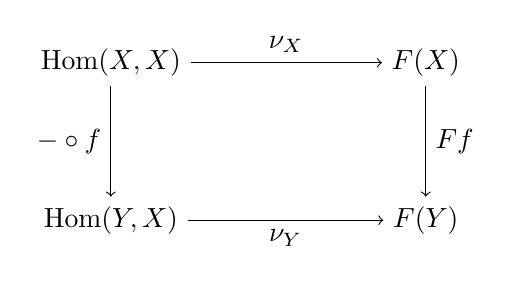
\begin{tikzpicture}

    \node (FX) at (4,0) {$F(X)$};
    \node (hY) at (0,-2) {$\operatorname{Hom}(Y,X)$};
    \node (hX) at (0,0) {$\operatorname{Hom}(X,X)$};
    \node (FY) at (4,-2) {$F(Y)$};
    \draw[->] (hX) -- node[left] {$- \circ f$} (hY);
    \draw[->] (FX) -- node[right] {$Ff$} (FY);
    \draw[->] (hX) -- node[above] {$\nu_X$} (FX); 
    \draw[->] (hY) -- node[below] {$\nu_Y$} (FY);
        \end{tikzpicture}
        \end{document}
